\chapterimage{Pictures/Ausberto/07_Modelagem.jpg}

\chapter{Modelagem do Sistema}

Neste capítulo descrevemos os comportamentos gerais do sistema, utilizando da abstração e da linguagem UML, de forma a simplificar o entendimento dos requisitos e como eles interagem com a aplicação, sem entrar de fato nos pormenores do desenvolvimento.

\section{Diagramas de Classes}
    O diagrama \ref{DiagClasses} se refere ao tipo de dados e funções que uma tag supostamente deveria comportar. Entretanto, nem tudo foi implementado.
    \begin{figure}[H]
        \begin{center}
            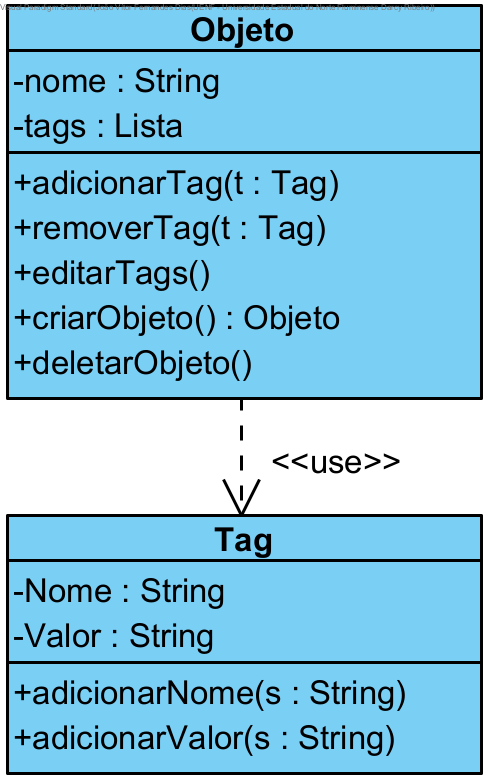
\includegraphics[width=12cm]{Pictures/JV/Diagramas/Sistema Tag - Diagrama de Classes.png}
            \caption{Diagrama de classes Tag} \label{DiagClasses}
        \end{center}
    \end{figure} 
\section{Diagramas Casos de uso}
    O diagrama \ref{DiagUso} representa as possibilidades de ações que os atores podem realizar no sistema
    \begin{figure}[H]
        \begin{center}
            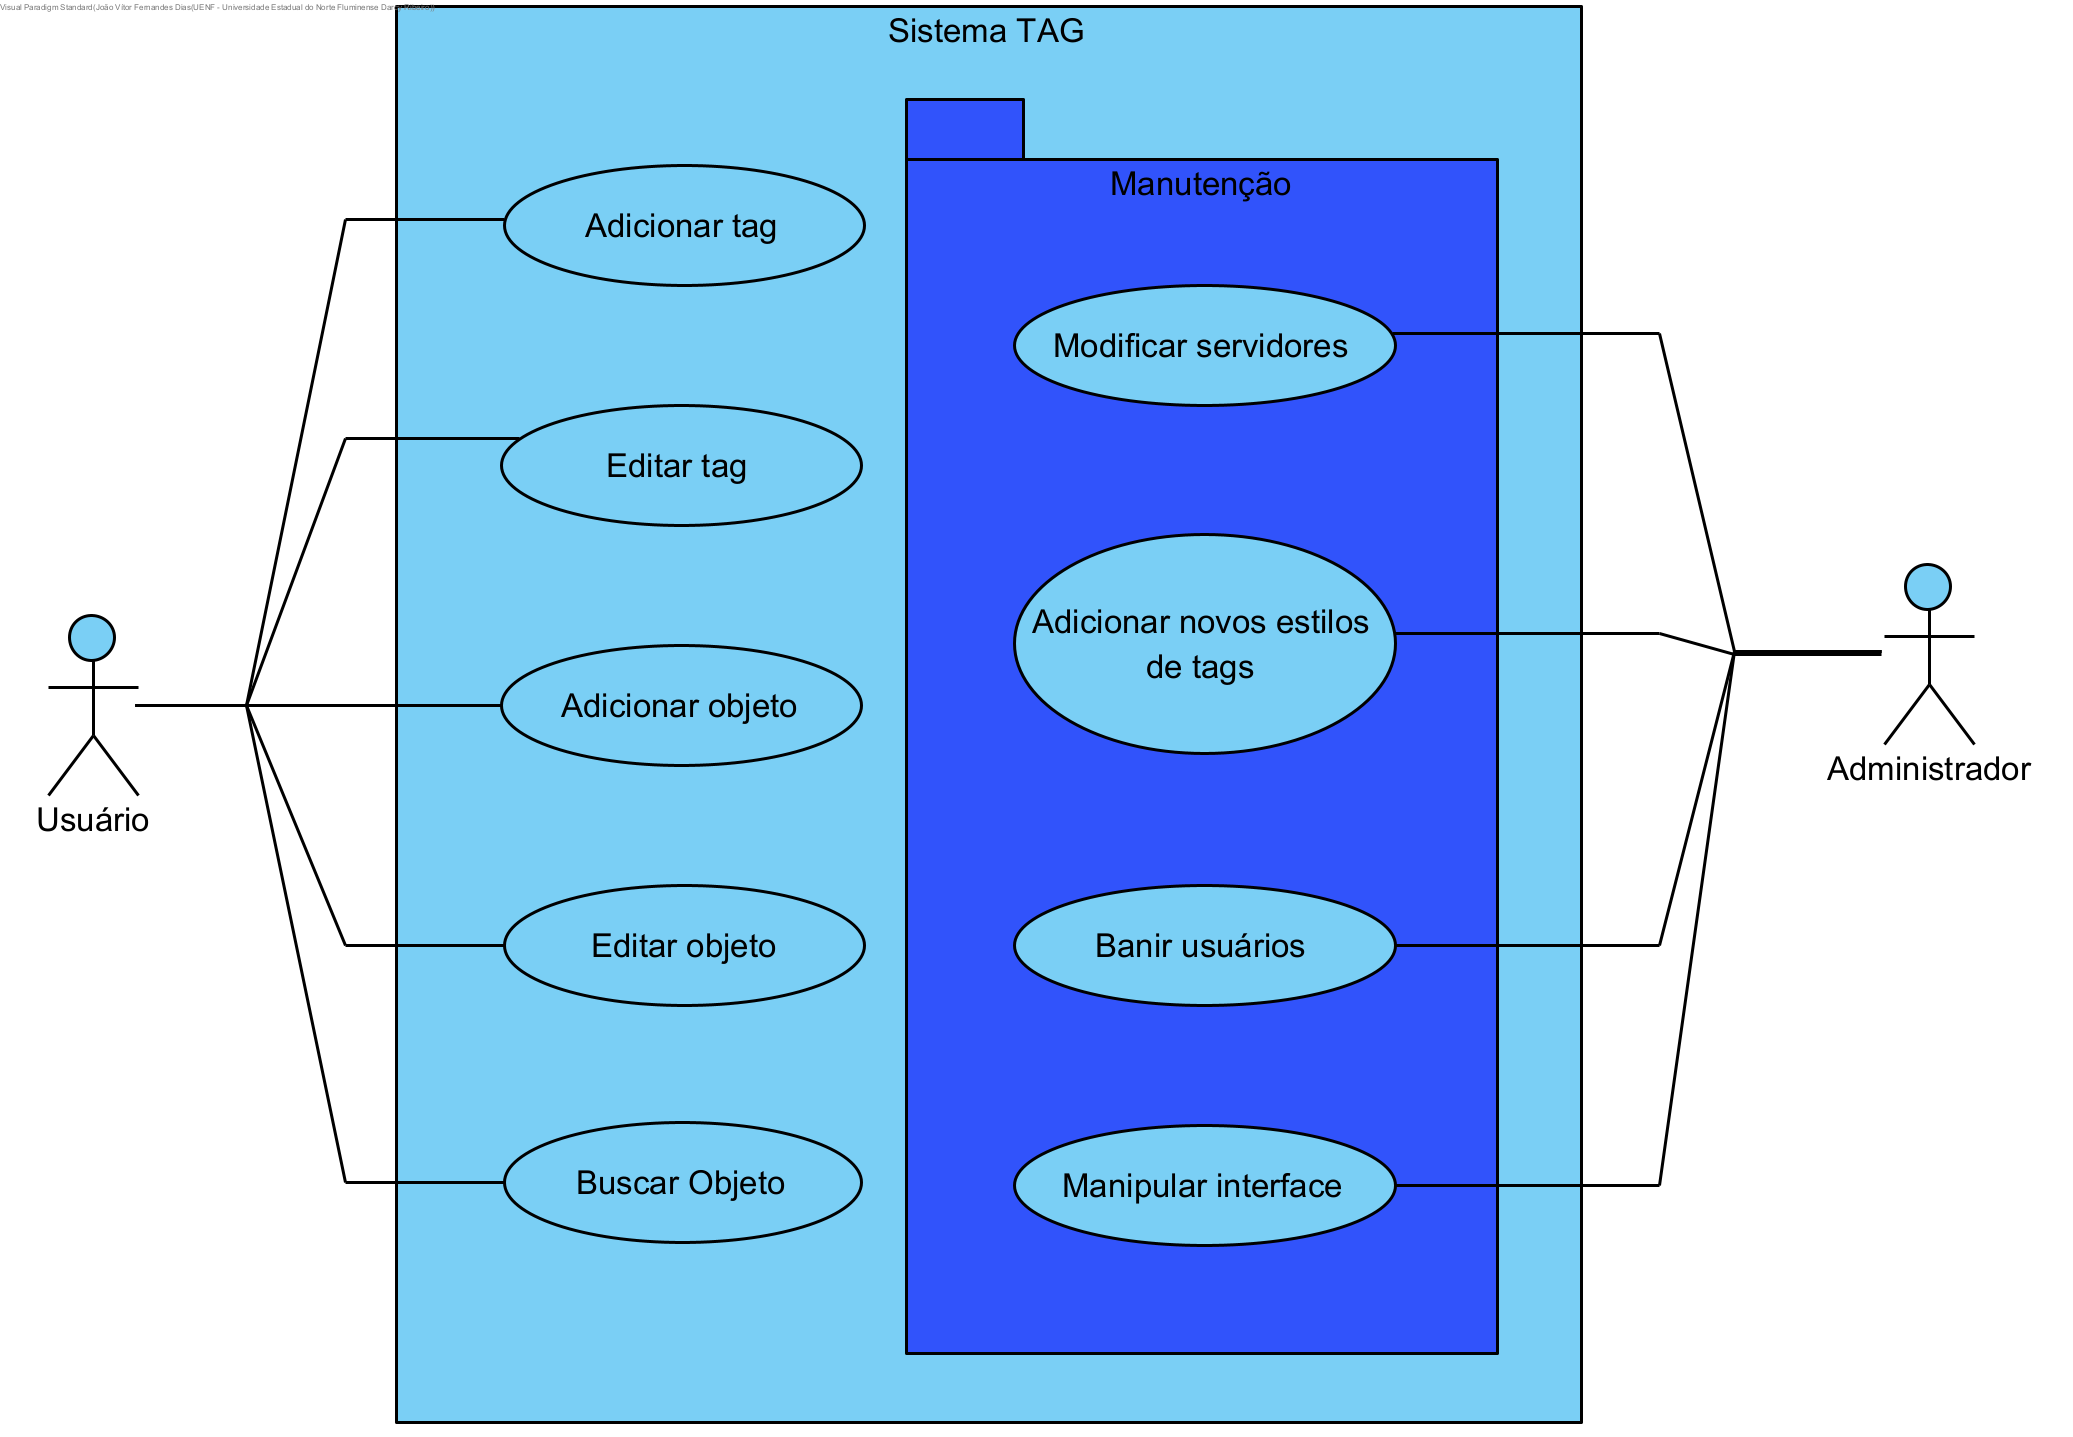
\includegraphics[width=12cm]{Pictures/JV/Diagramas/Sistema Tag - Casos de uso.png}
            \caption{Casos de uso do sistema Tag} \label{DiagUso}
        \end{center}
    \end{figure} 


\section{Diagramas Sequência}
    O diagrama de sequência \ref{DiagSeq} se refere à sequência de ações que ocorrem durante a tentativa de login.
    \begin{figure}[H]
        \begin{center}
            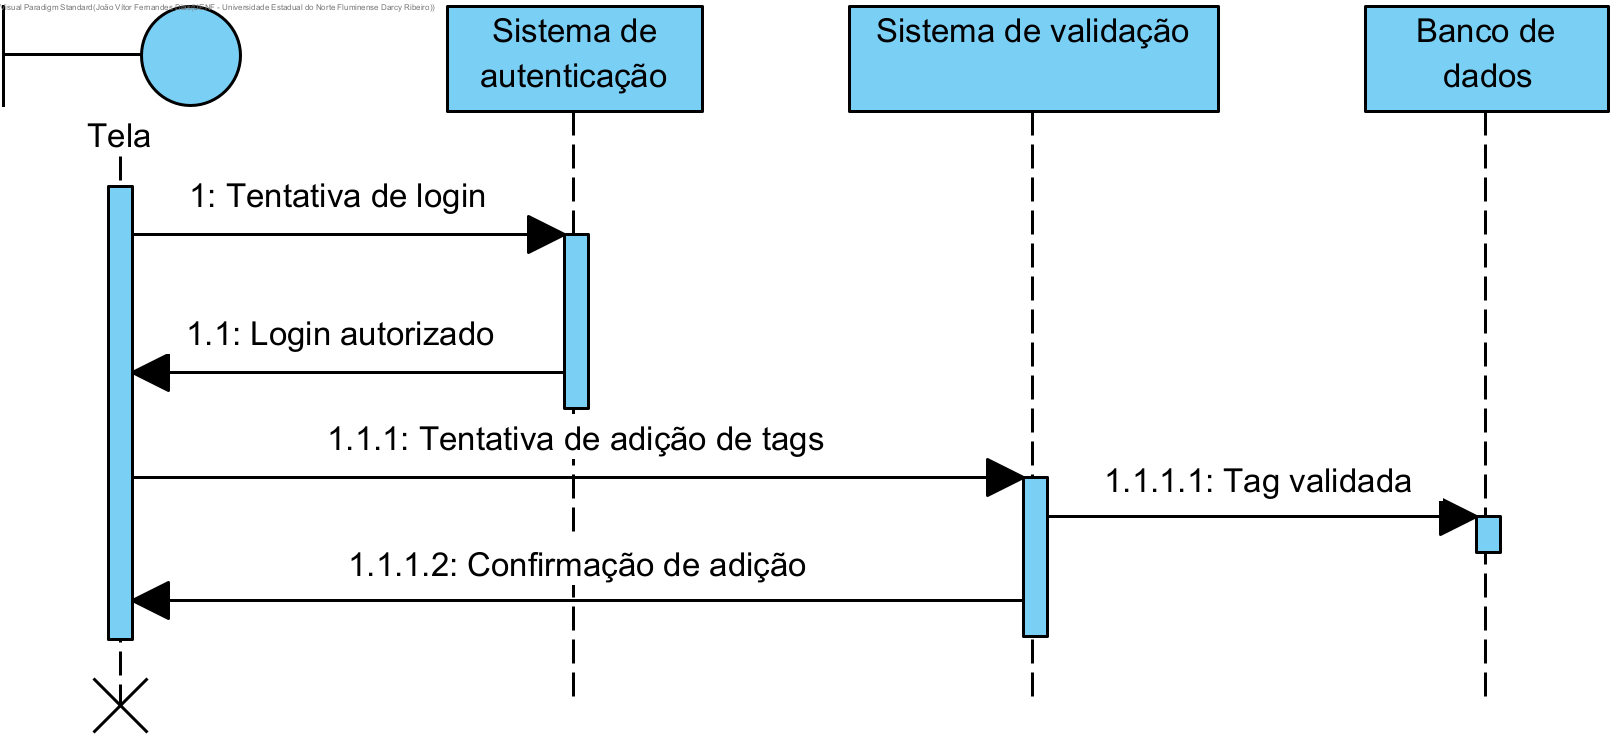
\includegraphics[width=12cm]{Pictures/JV/Diagramas/Sistema Tag - Diagrama de Sequencia.png}
            \caption{Diagrama de sequência do sistema Tag} \label{DiagSeq}
        \end{center}
    \end{figure} 

\begin{comment}
\section{Diagramas DFD}

    \begin{itemize}
      \item Diagrama de Contexto (Mostra o relacionamento e fluxo de dados entre o sistema e as entidades externas)
      \item Nível 1 do Sistema (O sistema como um todo junto com seus subsistemas)
      \item Nível 2
    \end{itemize}
    
\section{Diagramas E-R}
    As entidades são os objetos que participam do sistema
        
    \begin{figure}[H]
        \begin{center}
            \includegraphics[width=12cm]{Pictures/JV/Diagramas/}
            \caption{} \label{}
        \end{center}
    \end{figure} 
\section{Diagramas de Atividades}
    
    \begin{figure}[H]
        \begin{center}
            \includegraphics[width=12cm]{Pictures/JV/Diagramas/}
            \caption{} \label{}
        \end{center}
    \end{figure} 
\section{Diagramas Estado}
    
    \begin{figure}[H]
        \begin{center}
            \includegraphics[width=12cm]{Pictures/JV/Diagramas/}
            \caption{} \label{}
        \end{center}
    \end{figure} 
\end{comment}

\begin{comment}
    Prof. Dr. Ausberto S. Castro Vera
    UENF - CCT - LCMAT - Curso de Ciência da Computação
    Campos, RJ, 2022 
    Disciplina: Paradigma de Desenvolvimento Orientado a Objetos
    Aluno: João Vítor Fernandes Dias
\end{comment}